\chapter{РЕАЛИЗАЦИЯ}

\section{Программное обеспечение КУСД}

Работа КУСД, как было сказано ранее (стр. \pageref{reasonofwork}), полностью зависит от поддержки стека сетевых протоколов TCP/IP. Следовательно, основная часть данной работы направлена на создание программного обеспечения, реализующего поддержку стека сетевых протоколов.

В качестве инструмента реализации программного обеспечения использовался домашний компьютер с ОС Linux Ubuntu 16.04, на котором было установлен следующее ПО:
 \begin{itemize}
	\item набор GNU AVR Toolchain версии 4.9.2, в который входит\cite{avrtoolchain}:
	\begin{itemize}
		\item[•] компилятор avr-gcc, для комплиляции исходного кода на языке С/С++ в машинный язык микроконтроллеров семейства AVR;
		\item[•] набор ассемблера и компоновщика avr-binutils;
		\item[•] avr-libc --- подмножество стандартной библиотеки С с некоторыми специфичными для AVR функциями;
		\item[•] avr-gdb --- отладчик;
		\item[•] avrdude --- программа для загрузки/выгрузки/управления памятью программ и данных на МК AVR;
	\end{itemize}
	\item интегрированная среда разработки Elcipse версии 3.8.1 с плагином для разработки программ на МК AVR;
\end{itemize}

\section{Работа с Ethernet-контроллером}

Первоначально требовалось обеспечить передачу данных между Ethernet-контроллером и микроконтроллером ATmega328/P по шине SPI. Опираясь на таблицу \ref{spitabl}, а также на расположение выводов контроллера enc28j60 (рисунок \ref{fig:ethcontroller}), микроконтроллер был подключен к Ethernet-контроллеру. Соответсвие выходам микроконтроллера ATmega328/P и входам Ethernet-контроллера описано в таблице \ref{connection}. Стоит отметить что хоть Ethernet-контроллер в основном оперирует напряжением 3,3 В, на вход питания можно подавать 5 В и выше, поскольку на плате присутствует стабилизатор напряжения AMS1117\cite{voltageregulator}. После подключение убеждаемся в том, что на плату Ethernet-контроллера поступает питание по свечению светодида D1. 

\begin{table}[h!]
\caption{Соответствие выходам ATmega328/P и входам Ethernet-контроллера в данной работе}
\label{connection}
	\begin{tabular}{|p{40mm}|p{40mm}|p{40mm}|}
\hline
	Наименование соединения & Выход на ATmega328/P & Вход на Ethernet-контроллере \\
\hline
		MOSI & PB3 & MOSI (4)\\
\hline
		MISO & PB4 & MISO(10)\\
\hline
		SCLK & PB5 & SCK(9)\\
\hline
		SS & PB2 & CS (5)\\
\hline
\end{tabular}
\end{table}

Для взаимодействия с Ethernet-котроллером была написана библиотека на языке Си. Основной интерфейс данной библиотеки представлен в листинге \ref{lst:enc28j60header}. 

{\small{\lstinputlisting[language=C, caption=Интерфейс для взаимодействия с ENC28J60 по шине SPI\label{lst:enc28j60header}, inputencoding=cp1251, linerange={12-33}]{./src/enc28j60.h}}}

Алгоритм работы с Ethernet-контроллером следующий:
\begin{enumerate}
	\item настраиваем работу по шине SPI: 
		\begin{itemize}
			\item конфигурируем выходы микроконтроллера CS, MOSI, SCK на запись, а MISO на чтение;
			\item устанавливаем режим работы SPI интерфейса ATmega328/P как ``Мастер'';
			\item выставляем скорость работы шины SPI на максимальную;
			\item используем SPI режим 0 (CPOL=0, CPHA=0);
		\end{itemize}
	\item инициализируем ENC28J60:
		\begin{itemize}
			\item делаем ``мягкий сброс'' микросхемы;
			\item устанавливаем размер FIFO для приема данных (ERXST, ERXND), инициализируем указатель для чтения данных из FIFO (ERXRDPT);
			\item конфигурируем MAC: включаем аппаратное управление потоком, автоматическое выравнивание до 60 байт, автоматическое добавление контрольной суммы, устанавливаем MAC-адрес в регистрах MAADR;
			\item настраиваем PHY: устанавливаем дуплексный режим, настраиваем индикаторные светодиоды, отключаем loopback;
			\item разрешаем прием пакетов;
		\end{itemize}
	\item принимаем и отправляем пакеты;
\end{enumerate}

После того, как мы получили возможность обмениваться сырыми данными с другими Ethernet-устройствами, осталось написать протоколы канального, сетевого и транспортного уровня.

\section{Реализация протоколов стека TCP/IP}

Заголовки протокола Ethernet представлены в листинге \ref{lst:ethernethead}. 

{\small{\lstinputlisting[language=C, caption=Определение полей и заголовков для манипулирования Ethernet-кадрами\label{lst:ethernethead}, inputencoding=cp1251, linerange={13-13, 41-49}]{./src/lan.h}}}

Далее требовалось реализовать поддержку протокола сетевого уровня IP, что бы успешно взаимодействовать с другими хостами в сети, построенной на базе стека протоколов TCP/IP.
Заголовки протокола IP представлены в листинге \ref{lst:iphead}.

{\small{\lstinputlisting[language=C, caption=Определение полей и заголовков для манипулирования IP-датаграммами\label{lst:iphead}, inputencoding=cp1251, linerange={14-18, 82-98}]{./src/lan.h}}}

После того как определен и реализован некоторый базис, позволяющий передавать пакеты в локальной сети, небходимо связать канальный и сетевые уровни протоколом \textbf{ARP} (\textit{Address Resolution Protocol}). Это необходимо поскольку не существует другого явного алгоритма преобразования IP-адрес в MAC-адреса. 

Рассмотрим процедуру преобразования адресов при отправлении сообщения. Пусть один хост отправляет сообщение другому. Прикладной программе IP-адрес места назначения обычно известен. Для определения MAC-адреса просматривается ARP-таблица. Если для требуемого IP-адреса в ней присутствует MAC-адрес, то формируется и посылается пакет по соответствующему адресу. Если же с помощью APR-таблицы не удается преобразовать адрес, то выполняется следующее:
\begin{itemize}
	\item всем хостам в сети посылается пакет с ARP-запросом (с широковещательным MAC-адресом);
	\item исходящий IP-пакет ставится в очередь;
\end{itemize}

Каждый хост, принявший ARP-запрос, в своем ARP-модуле сравнивает собственный IP-адрес с IP-адресом в запросе. Если IP-адрес совпал, то прямо по MAC-адресу отправителя запроса посылается ответ, содержащий как IP-адрес ответившей машины, так и её MAC-адрес. Далее ответ принимается и заносится в ARP-таблицу, после чего отправляются все IP-пакеты которые были занесены в очередь на отправку к данному хосту. В противном случае (такой машины в сети нет) все IP-адреса по данному адресу отбрасываются. Пример ARP-таблицы отображен в таблице \ref{arptable}.

\begin{table}[h!]
\caption{Пример упрощенной ARP-таблицы}
\label{arptable}
	\begin{tabular}{|c|c|}
	\hline
	IP-адрес & MAC-адрес\\
	\hline
	192.168.0.1 & 30:b5:c2:cd:73:90 \\
	\hline
	192.168.0.102 & f4:f5:a5:73:da:b6 \\
	\hline
	192.168.0.103 & f8:32:e4:34:e7:61 \\
	\hline
	192.168.0.101 & 00:24:21:21:26:72 \\
	\hline
	\end{tabular}
\end{table}

Заголовки протокола ARP представлены в листинге \ref{lst:arphead}.

{\small{\lstinputlisting[language=C, caption=Определение полей и заголовков для протокола ARP\label{lst:arphead}, inputencoding=cp1251, linerange={20-20, 56-78}]{./src/lan.h}}}

Для тестирования работоспособности сетевого интерфейса (и вообще КУСД) не будет лишним реализовать поддержку протокола \textbf{ICMP}, а именно ICMP Echo запросы и ответы. Сам протокол ICMP служит для диагностики состояния сети. Echo-запросы имеют следующие поля:
\begin{enumerate}
	\item тип пакета: запрос (8) или ответ (0);
	\item код пакета --- 0 для Echo-запроса и ответа;
	\item контрольная сумма заголовка рассчитывается также, как и для заголовка IP-пакета;
	\item остальные поля устанавливаются на усмотрение хоста. Ответ должен содержать те же значения;
\end{enumerate}

Заголовки протокола ICMP (для Echo-запросов) представлены в листинге \ref{lst:icmpecho}.

{\small{\lstinputlisting[language=C, caption=Определение полей и заголовков для ICMP Echo запросов\label{lst:icmpecho}, inputencoding=cp1251, linerange={106-119}]{./src/lan.h}}}

Убедимся, что контроллер отвечает на Echo-запросы, отправив по его IP-адресу Echo-запрос. При этом, контроллер будет находится в домашней локальной сети по IP-адресу 192.168.0.140 и маской подсети 255.255.255.0. Отправим несколько Echo-запросов используя утилиту \textbf{ping} на одном из хостов в локальной сети (рисунок \ref{fig:echo-req}). При этом, будут считываться сообщения приходящие от самого контроллера по протоколу USART на домашний компьютер (рисунок \ref{fig:echo-reply-log}).

\begin{figure}[h!]
	\centering
		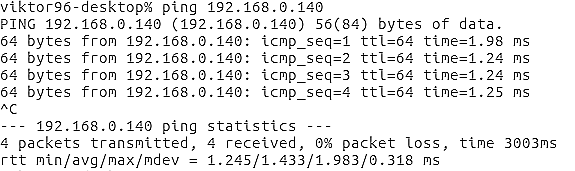
\includegraphics[scale=0.8]{img/icmp-req.png}
	\caption{Отправка Echo-запросов к КУСД\label{fig:echo-req}}
\end{figure}

\begin{figure}[h!]
	\centering
		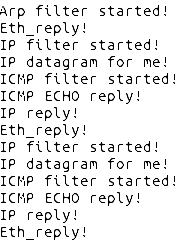
\includegraphics[scale=1.0]{img/echo-reply-log.png}
	\caption{Подтверждения о доставке Echo-запросов и ответа на них\label{fig:echo-reply-log}}
\end{figure}

Данные отладочные сообщают о том, что принятыей пакет прошел стадии обработки Ethernet фильтра, где контроллер распознал свой MAC-адрес, следом IP фильтра, где контроллер распознал свой IP-адрес, далее ICMP фильтра, в котором был распознан код и типа сообщения (код Echo-запроса, тип --- запрос). Далее последовал Echo-ответ, который собирался последовательно от уровня ICMP до Ethernet и был послан в сеть.

Как видно из рисунка \ref{fig:echo-req} по тому, что на все запросы были посланы ответы, стек протоколов от Ethernet до ICMP на данном контроллере работоспособен.



% range output - [firstline=*num*, lastline=*num*] or [linerange={(first1)-(last1), (first2)-(last2), ...}
%\small{\lstinputlisting[language=C, caption=main.c, inputencoding=cp1251]{./src/main.c}}
